\documentclass[12pt]{article}
\usepackage{graphicx}
\usepackage{xcolor}
\usepackage{geometry}
\geometry{margin=1in}

\begin{document}

\begin{center}
\includegraphics[width=0.4\textwidth]{iiitb_logo.png.jpg}
\end{center}

\begin{center}
\textbf{\Large Harshita N Kumar} \\
ID: COMETFWC052
\end{center}

\vspace{0.5cm}

{\color{blue}\section*{Question 11}}

Match the logic gates in Column A with their equivalents in Column B.

\vspace{0.5cm}

\begin{center}
\begin{tabular}{|c|c|}
\hline
\textbf{Column-A} & \textbf{Column-B} \\
\hline
1. AND GATE & P. XOR GATE \\
2. OR GATE  & Q. XNOR GATE \\
3. NOT GATE & R. NAND GATE \\
\hline
\end{tabular}
\end{center}

\vspace{0.3cm}

\begin{center}
\textbf{TABLE 11: Table-1}
\end{center}

\vspace{0.5cm}

a) P-2, Q-4, R-1, S-3 \hspace{1cm}
b) P-4, Q-2, R-1, S-3

\vspace{0.3cm}

c) P-2, Q-4, R-3, S-1 \hspace{1cm}
d) P-4, Q-2, R-3, S-1


\vspace{0.8cm}

{\color{blue}\section*{Question Analysis}}

The AND gate produces output 1 only when both inputs are 1.  
The NAND gate is the complement of AND, meaning $NAND = (A \cdot B)'$.  

The XOR gate produces output 1 when inputs are different.  
The XNOR gate is the complement of XOR.  

The NOT gate performs inversion.  

After comparing logical equivalences and understanding the 
behavior of each gate, we identify the correct matching.


\vspace{0.8cm}

\newpage
{\color{blue}\section*{Truth Table}}

AND Gate: $Q = A \cdot B$

\begin{center}
\begin{tabular}{|c|c|c|}
\hline
A & B & A.B \\
\hline
0 & 0 & 0 \\
0 & 1 & 0 \\
1 & 0 & 0 \\
1 & 1 & 1 \\
\hline
\end{tabular}
\end{center}

NAND Gate: $Q = (A \cdot B)'$

\begin{center}
\begin{tabular}{|c|c|c|}
\hline
A & B & NAND \\
\hline
0 & 0 & 1 \\
0 & 1 & 1 \\
1 & 0 & 1 \\
1 & 1 & 0 \\
\hline
\end{tabular}
\end{center}


\vspace{0.8cm}

{\color{blue}\section*{Hardware Implementation}}

The hardware setup consists of Arduino UNO, IC 7447, 
common anode 7-segment display, breadboard and jumper wires.  

The logical output is generated from Arduino and converted into 
BCD format. The 7447 decoder drives the 7-segment display 
to visually represent the output.


\begin{center}
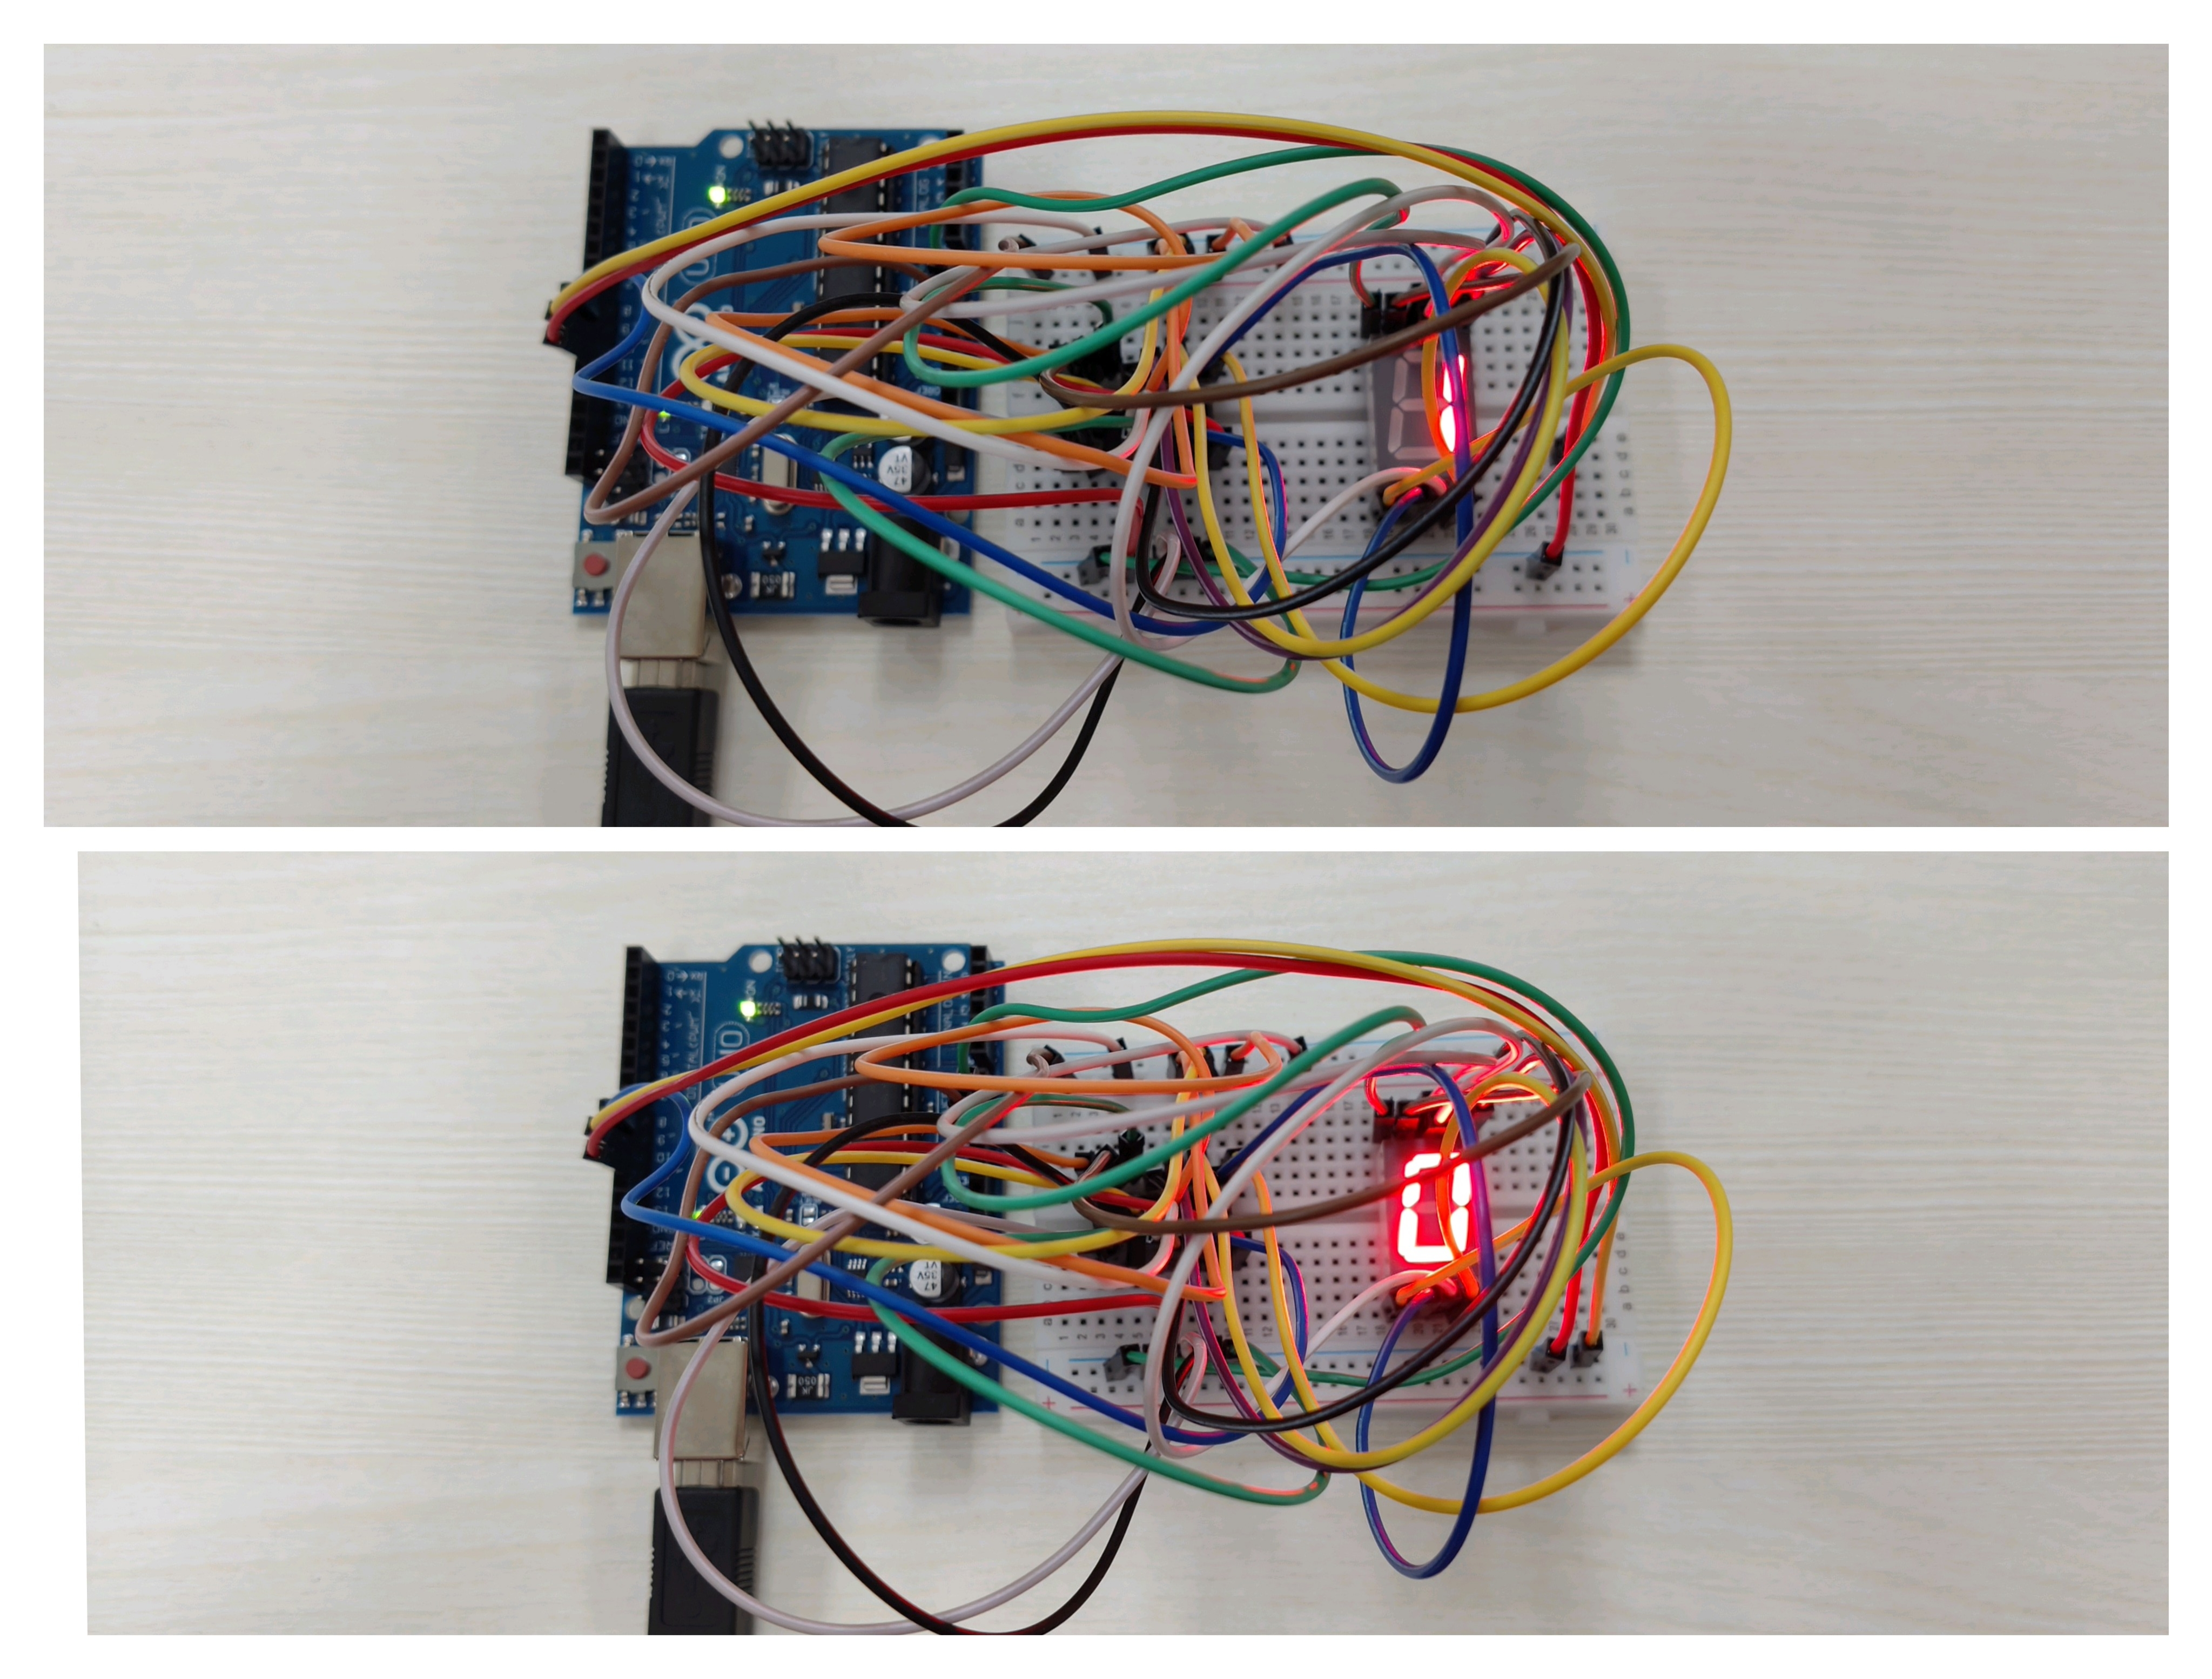
\includegraphics[width=0.8\textwidth]{hardware.jpg}
\end{center}


\vspace{0.8cm}

{\color{blue}\section*{Required Components}}

\begin{itemize}
\item Arduino UNO
\item IC 7447
\item Common Anode 7-Segment Display
\item Breadboard
\item Jumper wires
\end{itemize}


\vspace{0.8cm}

{\color{blue}\section*{Pin Connections}}

Pin 16 $\rightarrow$ 5V  
Pin 8 $\rightarrow$ GND  
Pin 3,4,5 $\rightarrow$ 5V  

Common Anode $\rightarrow$ 5V  

Segment pins connected from 7447 output pins 
through current limiting resistors.


\vspace{0.8cm}

{\color{blue}\section*{Logic Description}}

The NAND logic is implemented using digital inputs.

Expression: $Q = (A \cdot B)'$

The output remains HIGH for all cases except when 
both inputs are HIGH.


\vspace{0.8cm}

{\color{blue}\section*{Conclusion}}

The truth table verification and logical analysis confirm 
the equivalence of the gates.

\bigskip

\begin{center}
\textbf{\Large The correct option is: (c) P-2, Q-4, R-3, S-1}
\end{center}

\bigskip

Thus, the matching is verified successfully.


\end{document}
